\documentclass[final]{beamer}

\usepackage[size=custom,width=91.44,height=60.96,scale=0.80]{beamerposter}
\usepackage{graphicx}
\usepackage{booktabs}
\usepackage{array}
\usepackage{hyperref}
\usepackage{xcolor}

\definecolor{deepblue}{HTML}{1F4E79}
\definecolor{accentred}{HTML}{D1495B}
\definecolor{textgray}{HTML}{333333}

\setbeamercolor{headline}{bg=deepblue, fg=white}
\setbeamercolor{block title}{bg=deepblue, fg=white}
\setbeamercolor{block body}{bg=white, fg=textgray}
\setbeamercolor{normal text}{fg=textgray}
\setbeamertemplate{navigation symbols}{}
\setbeamertemplate{block begin}{
  \vskip0.42em
  \begin{beamercolorbox}[rounded=true,shadow=false,leftskip=0.65em,colsep*=0.42em]{block title}
    \usebeamerfont*{block title}\insertblocktitle
  \end{beamercolorbox}
  \begin{beamercolorbox}[rounded=true,shadow=false,leftskip=0.65em,rightskip=0.65em,colsep*=0.55em]{block body}
}
\setbeamertemplate{block end}{
  \end{beamercolorbox}
}

\title{\textbf{Re-implementing PatchTST for Long-term Multivariate Forecasting}}
\author{Mingde Zhou (zm339) \quad CS 4782 Final Project}
\institute{\href{https://github.com/MingdeZhou/PatchTST}{github.com/MingdeZhou/PatchTST}}

\begin{document}
\begin{frame}[t]

\begin{beamercolorbox}[wd=\paperwidth,sep=0pt]{headline}
  \begin{minipage}[t][2.45in][c]{\paperwidth}
    \hspace*{1.0in}
    \begin{minipage}{34in}
      {\fontsize{33}{38}\selectfont \inserttitle \par}
      \vspace{0.22in}
      {\fontsize{18}{22}\selectfont \insertauthor \hfill \insertinstitute \par}
    \end{minipage}
  \end{minipage}
\end{beamercolorbox}

\vspace{0.18in}
\begin{columns}[t,totalwidth=33.2in]

\begin{column}{15.8in}

\begin{block}{Motivation and Scope}
\textbf{Question.} Can a vanilla Transformer work well for long-term time-series forecasting if the input representation is designed correctly?

\vspace{0.25em}
\textbf{Paper.} PatchTST argues that two design choices are central:
\begin{itemize}
  \item \textbf{Patching:} use short temporal segments as tokens instead of individual timestamps.
  \item \textbf{Channel independence:} process each variable as a univariate sequence while sharing Transformer weights.
\end{itemize}

\vspace{0.25em}
\textbf{Reproduction target.} Supervised multivariate Weather forecasting from Table 3, using PatchTST/42-style settings.

\vspace{0.25em}
\textbf{What was reimplemented.}
\begin{itemize}
  \item Supervised PatchTST core in PyTorch, keeping \(\texttt{[B,L,C]}\rightarrow\texttt{[B,T,C]}\).
  \item RevIN-style normalization, patch extraction, shared Transformer encoding, and flatten prediction head.
  \item Train/test and checkpoint-load inference paths.
\end{itemize}
\end{block}

\begin{block}{Method}
The model treats each multivariate window \(X\in\mathbb{R}^{B\times L\times C}\) as a collection of channel-specific temporal sequences. Each channel is normalized independently, divided into overlapping temporal patches, encoded with one shared Transformer, and projected to the target horizon.

\vspace{0.2em}
\begin{center}
\begin{tabular}{>{\bfseries}p{2.8in}p{11.8in}}
\toprule
Normalize & RevIN-style per-instance statistics over the time dimension. \\
Patch & Repeat-pad the last value, then extract overlapping \(P=16\), \(S=8\) temporal patches. \\
Encode & Fold channels into the batch dimension, so all variables share one temporal Transformer encoder. \\
Predict & Flatten encoded patches and apply a shared linear head to produce each channel's forecast. \\
\bottomrule
\end{tabular}
\end{center}

\vspace{0.15em}
\textbf{Key idea.} Patches make tokens locally meaningful, while channel independence avoids early mixing of heterogeneous weather variables.
\end{block}

\begin{block}{Experimental Setup}
\begin{center}
\begin{tabular}{>{\bfseries}p{3.0in}p{11.6in}}
\toprule
Dataset & Weather benchmark, 21 variables, 52,696 timestamps \\
Input & Look-back window \(L=336\) \\
Outputs & Horizons \(T=\{96,192,336,720\}\) \\
Metrics & MSE and MAE \\
Training budget & 10 epochs, patience 3 \\
\bottomrule
\end{tabular}
\end{center}
\end{block}

\begin{block}{Reading the Results}
\begin{itemize}
  \item The shape of the curve is reproduced: both MSE and MAE rise monotonically with horizon.
  \item MSE gap stays within roughly \(2\%\)--\(4\%\), and MAE gap stays within roughly \(1\%\)--\(5\%\).
  \item The small gap is expected because this reproduction used a shorter training budget than the original paper.
  \item Output arrays have shape \(\texttt{[batch, pred\_len, 21]}\), and all reported metrics are finite.
\end{itemize}
\end{block}

\begin{block}{Takeaways}
\begin{itemize}
  \item The supervised PatchTST result is reproducible at small scale on real Weather data.
  \item Most modeling value comes from tokenization and channel handling, not from exotic attention variants.
  \item Natural next steps are longer training, more datasets, patch-size ablations, and explicit cross-channel modeling.
\end{itemize}
\end{block}

\begin{block}{Reference}
\small
Nie et al. \textit{A Time Series is Worth 64 Words: Long-term Forecasting with Transformers}. ICLR 2023.
\end{block}

\end{column}

\begin{column}{16.6in}

\begin{block}{Reproduction Results}
\begin{center}
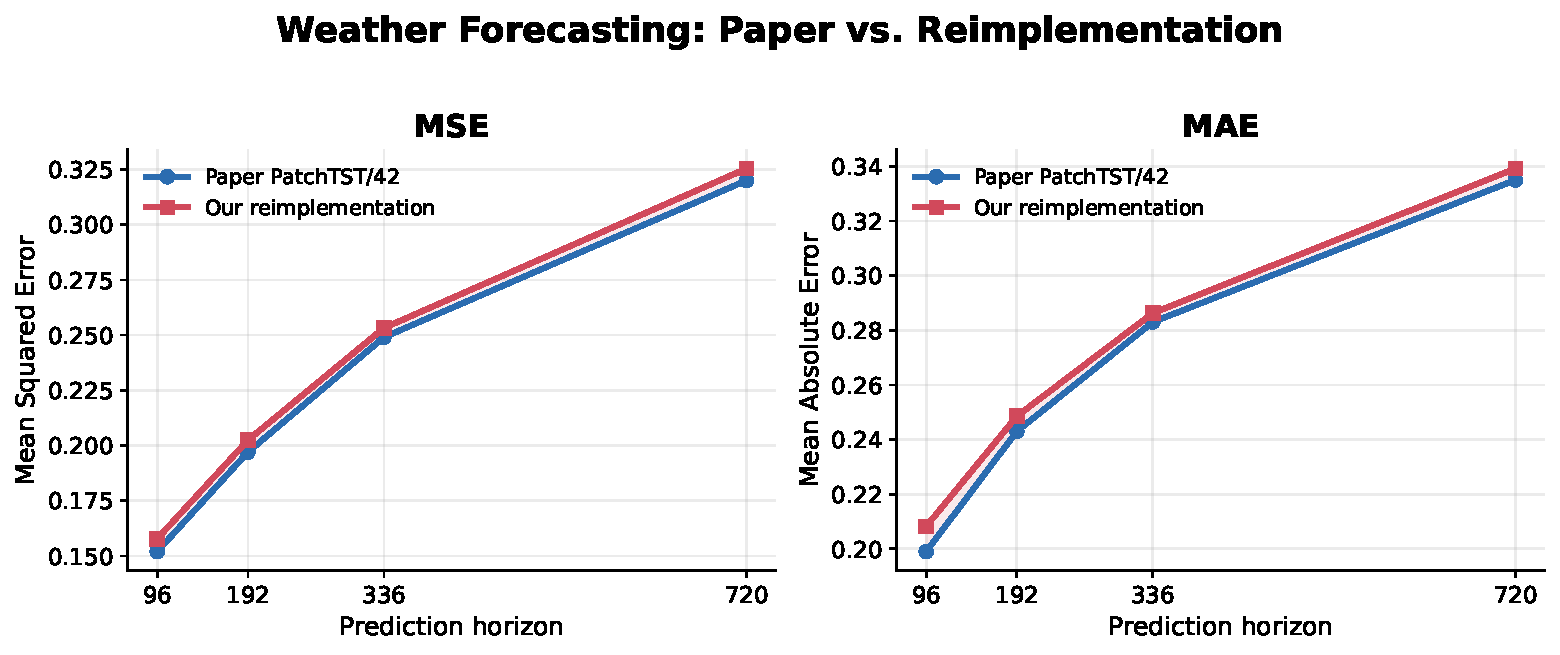
\includegraphics[width=13.7in]{images/paper_vs_reimplementation.pdf}
\end{center}
\vspace{-0.05in}
The reproduced Weather curves track the paper across all four long-horizon settings.
\end{block}

\begin{block}{Result Gap Analysis}
\begin{center}
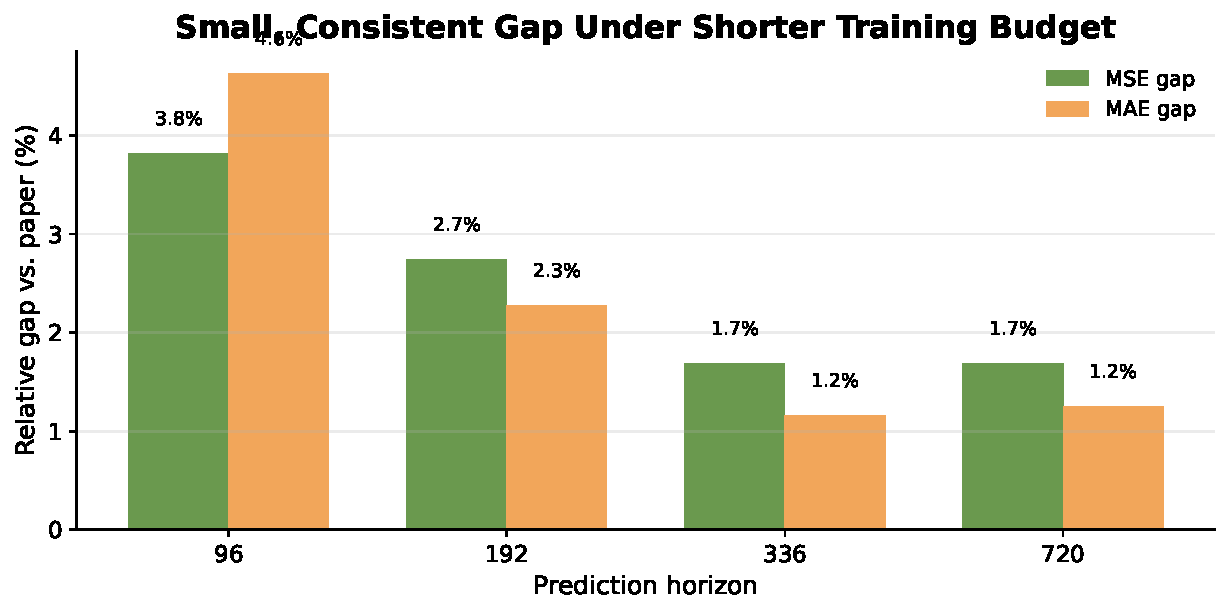
\includegraphics[width=12.7in]{images/relative_gap.pdf}
\end{center}
\vspace{-0.1in}
The relative gap remains small and consistent under a shorter training budget.
\end{block}

\begin{block}{Numerical Summary}
\begin{center}
\normalsize
\begin{tabular}{rrrrr}
\toprule
Horizon & Paper MSE & Ours MSE & Paper MAE & Ours MAE \\
\midrule
96  & 0.152 & 0.1578 & 0.199 & 0.2082 \\
192 & 0.197 & 0.2024 & 0.243 & 0.2485 \\
336 & 0.249 & 0.2532 & 0.283 & 0.2863 \\
720 & 0.320 & 0.3254 & 0.335 & 0.3392 \\
\bottomrule
\end{tabular}
\end{center}
\end{block}

\end{column}

\end{columns}

\end{frame}
\end{document}
